
\documentclass[a4paper,12pt]{article} % тип документа

% Поля страниц
\usepackage[left=2.5cm,right=2.5cm, top=2cm,bottom=2cm,bindingoffset=0cm]{geometry}

%Пакет дял таблиц   
\usepackage{multirow} % Слияние строк в таблице
\newcommand{\eds}{\ensuremath{ \mathscr{E}}}
\newcommand{\ga}{\ensuremath{\gamma}}
\usepackage{tikz} 
\usepackage{array,tabularx,tabulary,booktabs} % Дополнительная работа с таблицами
\usepackage{longtable}  % Длинные таблицы
\usepackage{multirow} % Слияние строк в таблице
%Отступ после заголовка    
\usepackage{indentfirst}


% Рисунки
\usepackage{subcaption,floatrow,graphicx,calc}
\usepackage{wrapfig}

% Создаёем новый разделитель
\DeclareFloatSeparators{mysep}{\hspace{1cm}}

% Ссылки?
\usepackage{hyperref}
%\usepackage[rgb]{xcolor}
%  Русский язык
\usepackage[T2A]{fontenc}			% кодировка
\usepackage[utf8]{inputenc}			% кодировка исходного текста
\usepackage[english,russian]{babel}	% локализация и переносы


% Математика
\usepackage{amsmath,amsfonts,amssymb,amsthm,mathtools, mathrsfs, wasysym}

\author{Гаврилин Илья\\
	Добровольская Ксения\\
	Б01-110}
\title{\textbf{Лабораторная работа 5.5.5\\ 
		Компьютерная сцинтилляционная $\gamma$ спектрометрия}}
	
\begin{document}
	\maketitle
	
	\paragraph*{Цель работы:} В данной работе предполагается изучить спектр гамма-излучений для образцов $ \mathrm{^{22}Na, ^{137}Cs, ^{60}Co }$, найти для них пики полного поглощения и обратного рассеяния.
	
	
	
	\section{Теоретическое введение}
	
	Основная задача спектрометрических измерений заключается в определении энергии, интенсивности дискретных гамма-линий от различных гамма-источников и их идентификации.
	
	Основными процессами взаимодействия гамма-излучения с веществом являются фотоэффект, эффект Комптона и образование электрон-позитронных пар. Каждый из этих процессов вносит свой вклад в образование наблюдаемого спектра. Образующиеся при этих процессах электроны испытывают большое количество неупругих соударений с молекулами и атомами среды. Неупругие соударения могут сопровождаться как ионизацией, так и возбуждением молекул или атомов среды. В промежуточных же стадиях (при переходах возбужденных молекул или атомов в основное состояние, при рекомбинации электрических зарядов и т.п.) в веществе возникают кванты света различных длин волн, присущих данному веществу.
	
	При \textbf{фотоэффекте} кинетическая энергия электрона $ T_e = E_\ga - I_i $, где $ I_i $ --- энергия ионизации $ i $-той оболочки атома. Фотоэффект особенно существенен для тяжелых веществ, где он идет с заметной вероятностью даже при высоких энергиях гамма-квантов. В легких веществах фотоэффект становится заметен лишь при относительно небольших энергиях гамма-квантов. Наряду с фотоэффектом, при котором вся энергия гамма-кванта передается атомному электрону, взаимодействие гамма-излучения со средой может приводить к его рассеянию, т.е. отклонению от первоначального направления распространения на некоторый угол.
	
	При \textbf{эффекте Компотна} происходит упругое рассеяние фотона на свободном электроне, сопровождающееся изменением длины волны фотона (реально этот процесс происходит на слабо связанных с атомом внешних электронах). Максимальная энергия образующихся комптоновских электронов соответствует рассеянию гамма-квантов на $ 2\pi $ и равна
	
	\begin{equation}\label{E_compton}
		E_{с \_ max} = \dfrac{\hbar \omega}{1 + \dfrac{m_ec^2}{2\hbar\omega}}
	\end{equation}
	
	При достаточно высокой энергии гамма-кванта наряду с фотоэффектом и эффектом Комптона может происходить третий вид взаимодействия гамма-квантов с веществом – \textbf{образование электрон-позитронных пар}. При этом если процесс образования пары идет в кулоновском поле ядра или протона, то энергия образующегося ядра отдачи оказывается весьма малой, так что пороговая энергия гамма-кванта, необходимая для образования пары, практически совпадает с удвоенной энергией покоя электрона $ Е_0 = 2m_ec^2 =1,022  $МэВ.
	
	Появившийся в результате процесса образования пар электрон теряет свою энергию на ионизацию среды. Таким образом, вся энергия электрона остается в детекторе. Позитрон будет двигаться до тех пор, пока практически не остановится, а затем аннигилирует с электроном среды, в результате чего появятся два гамма-кванта. Т.е., кинетическая энергия позитрона также останется в детекторе. Далее возможны три варианта развития событий:
	
	а) оба родившихся гамма-кванта не вылетают из детектора, и тогда вся энергия первичного гамма-кванта останется в детекторе, а в спектре появится пик с $ E = E_\gamma $;
	
	б) один из родившихся гамма-квантов покидает детектор, и в спектре появляется пик, соответствующий энергии $  Е = Е_\gamma - E0 $, где $ Е_0 = m_ec^2 = $ 511 кэВ;
	
	в) оба родившихся гамма-кванта покидают детектор, и в спектре появля- ется пик, соответствующий энергии $  Е = Е_\gamma - 2E0 $, где $ 2Е_0 = 2m_ec^2 = $ 1022 кэВ;
	
	Таким образом, любой спектр, получаемый с помощью гамма-спектрометра, описывается несколькими компонентами, каждая из которых связана с определенным физическим процессом. Как описано выше, основными физическими процессами взаимодействия гамма-квантов с веществом являются фотоэффект, эффект Комптона и образование электрон-позитронных пар, и каждый из них вносит свой вклад в образование спектра. Помимо этих процессов, добавляются экспонента, связанная с наличием фона, пик характеристического излучения, возникающий при взаимодействии гамма-квантов с окружающим веществом, а также пик обратного рассеяния, образующийся при энергии квантов $ Е_\gamma \gg mc^22/2 $ в результате рассеяния гамма-квантов на большие углы на материалах конструктивных элементов детектора и защиты. Положение пика обратного рассеяния определяется по формуле ($ E $ --- энергия фотопика):
	
	\begin{equation}\label{Eobr}
		E_{обр} = \dfrac{E}{1 + \dfrac{2E}{mc^2}}
	\end{equation}
	
	%	\section{Экспериментальная установка}
	%	
	Энергетическим разрешением спектрометра называется величина
	
	\begin{equation}\label{Ri = dE/E}
		R_i = \dfrac{\Delta E_i}{E_i}
	\end{equation}
	
	т.е. отношение ширины пика полного поглощения (измеренной на полувысоте) к регистрируемой энергии пика поглощения. Это значение $ E_i \propto \overline{n_i} $ --- числу частиц на выходе ФЭУ. При этом  $ \Delta E_i \propto \overline{\Delta n_i} = \sqrt{\overline{n_i}} $ --- ширина пика пропорциональна среднеквадратичной флуктуации, которая равна корню из числа частиц. Таким образом, наша формула \eqref{Ri = dE/E} примет вид
	
	\begin{equation}\label{Ri = c/E}
		R_i = \dfrac{\mathrm{const}}{\sqrt{E_i}}
	\end{equation}
	\section{Ход работы}
	Проведем измерения гамма-спектров для $ \mathrm{^{22}Na, ^{137}Cs, ^{60}Co}$, а также измерение фона. Получаем зависимость счета на сцинтилляторе $ N'_\text{ч} $ от номера канала $ N $. 
	\begin{equation}\label{}
		N_{Na\_1} = 718.1, \quad N_{Na\_2} = 1695.2
	\end{equation}
	
	Мы знаем, что этим пикам соответствуют табличные значения энергии 511, 1275 кэВ соответственно. Тогда проведем калибровку спектрометра, построив линейную зависимость энергии гамма-кванта от номера канала $ E_j = f(N_j) $. Результат калибровки:
	
	\begin{equation}\label{}
		E_j = (-57.690 + 0.789N_i ) \; \text{кэВ}
	\end{equation}
	С помощью полученной зависимости переведем все полученные значения каналов в энергии, а счет сцинтиллятора отнормируем по времени, получив число частиц за секунду $ N_\text{ч} = \dfrac{N'_\text{ч}}{t} $. Погрешность счета подсчитаем по формуле 
	
	\begin{equation}\label{}
		\sigma_{N_\text{ч}} = N_\text{ч}  \dfrac{\sqrt{N'_\text{ч}}}{N'_\text{ч}} = \dfrac{\sqrt{N'_\text{ч}}}{t}
	\end{equation}

	С помощью ПО компьютера экспериментальной установки получим значения пиков полного поглощения и их ширины.
	\begin{figure}[H]
		\centering
		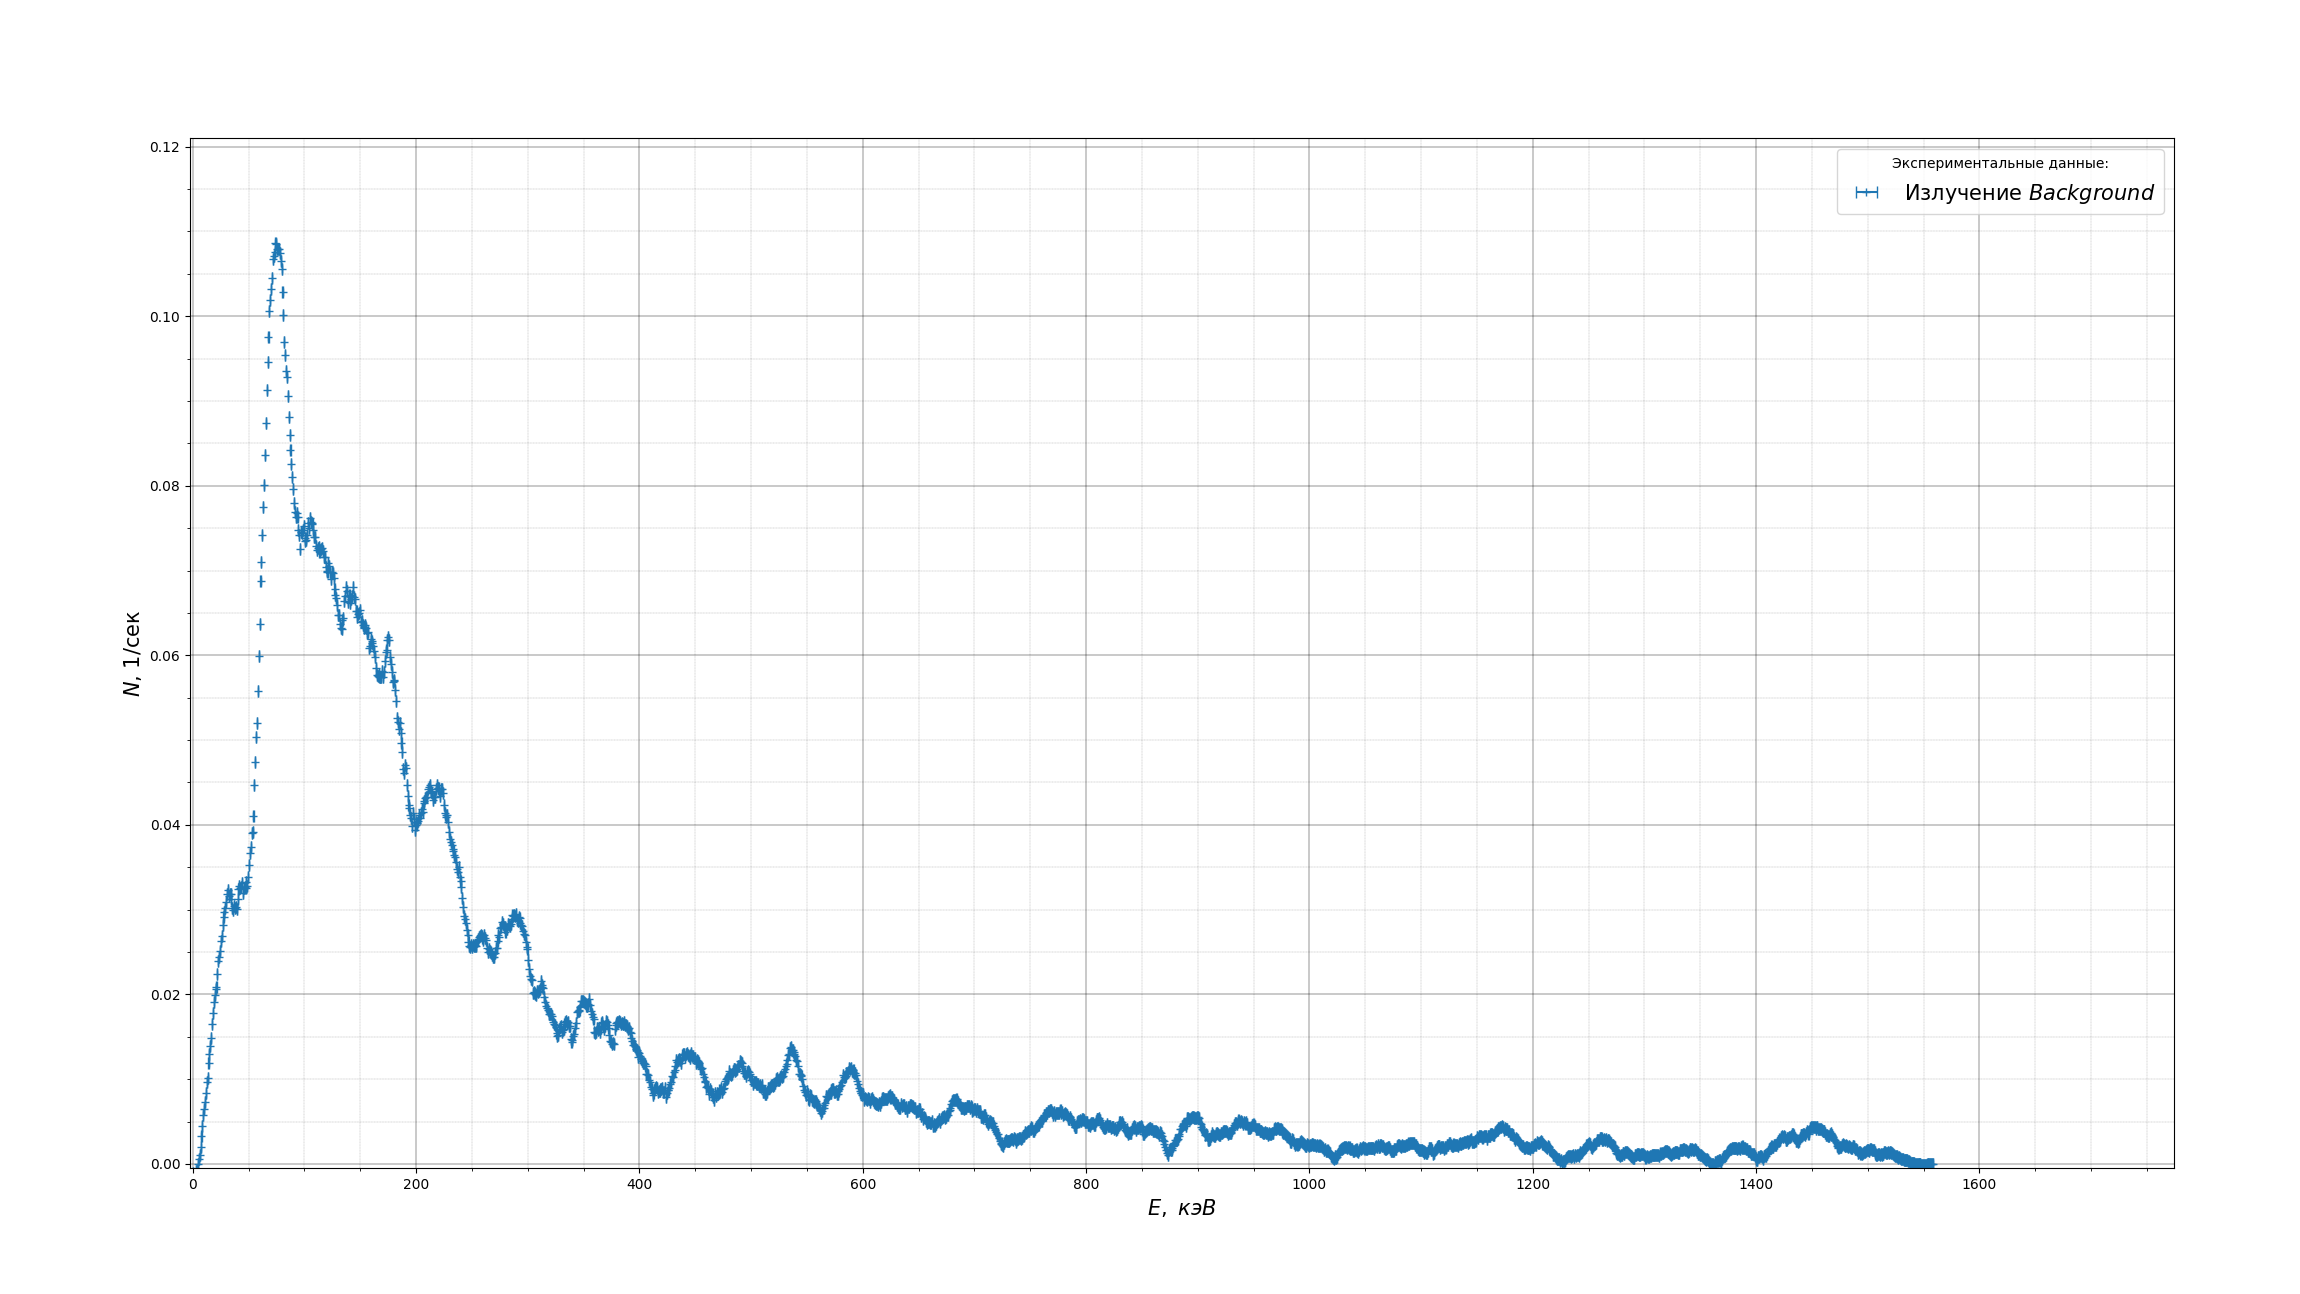
\includegraphics[width=0.95\linewidth]{Bg}
		\caption{Фоновое излучение}
		\label{fig:bg}
	\end{figure}
	Получив спектр фонового излучения, в дальнейшем будем вычитать его из спектров образцов. Построим спектры изучаемых образцов.
	\begin{figure}[H]
		\centering
		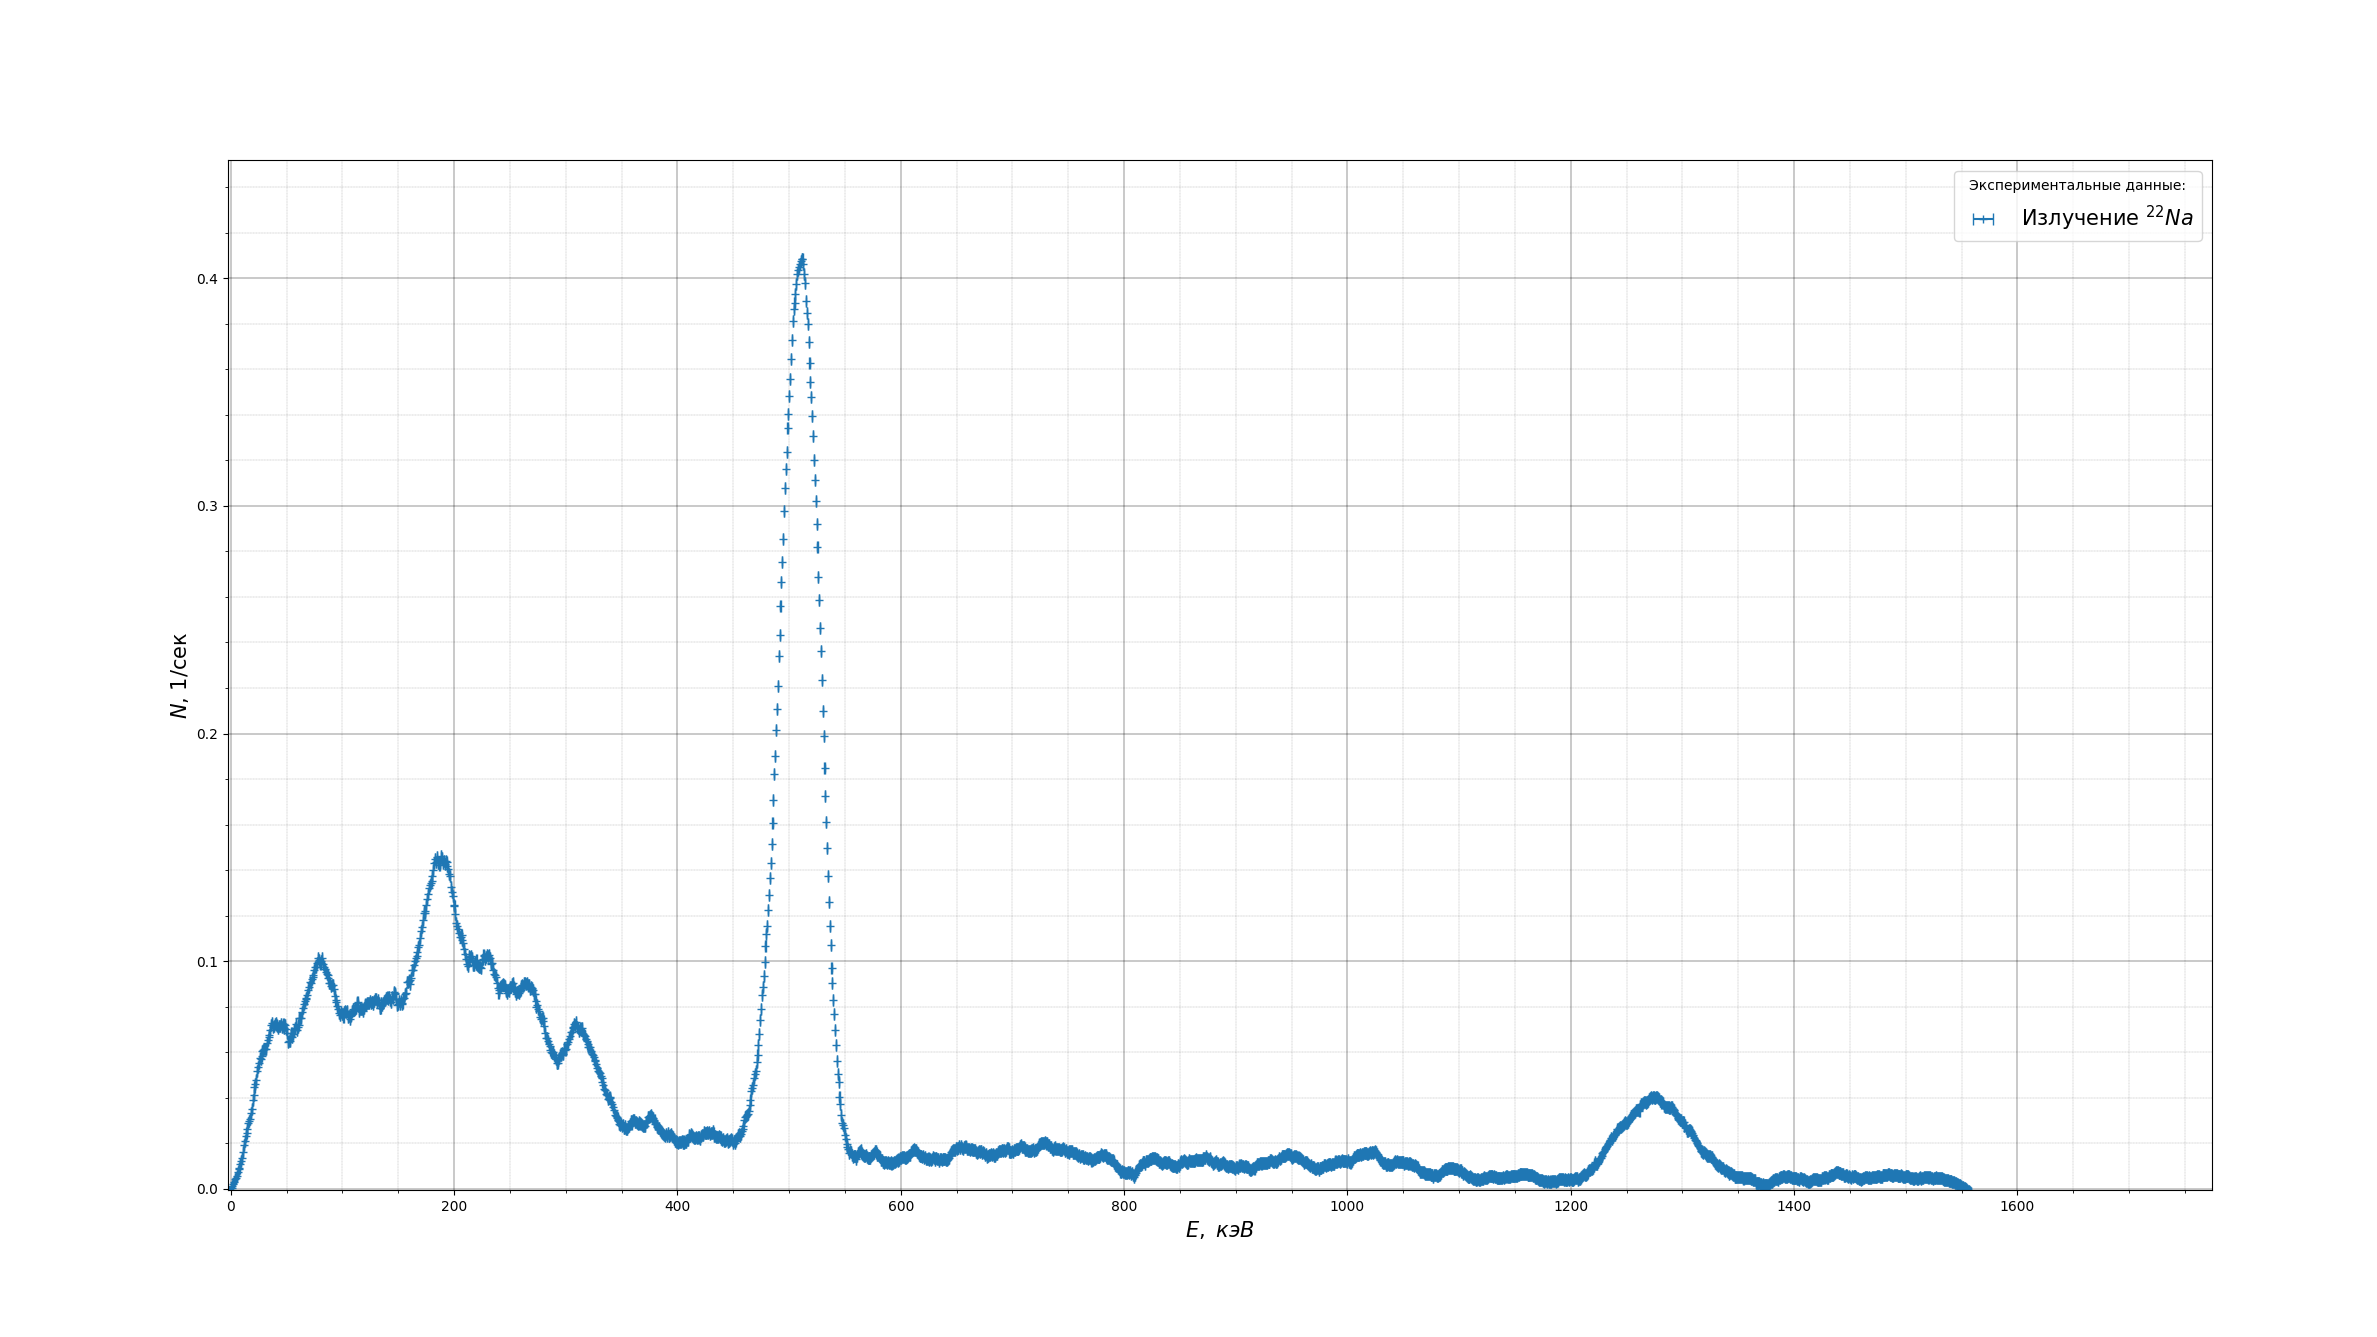
\includegraphics[width=0.95\linewidth]{Na_22}
		\caption{Спектр $^{22}Na$}
		\label{fig:na22}
	\end{figure}
	\begin{figure}[H]
		\centering
		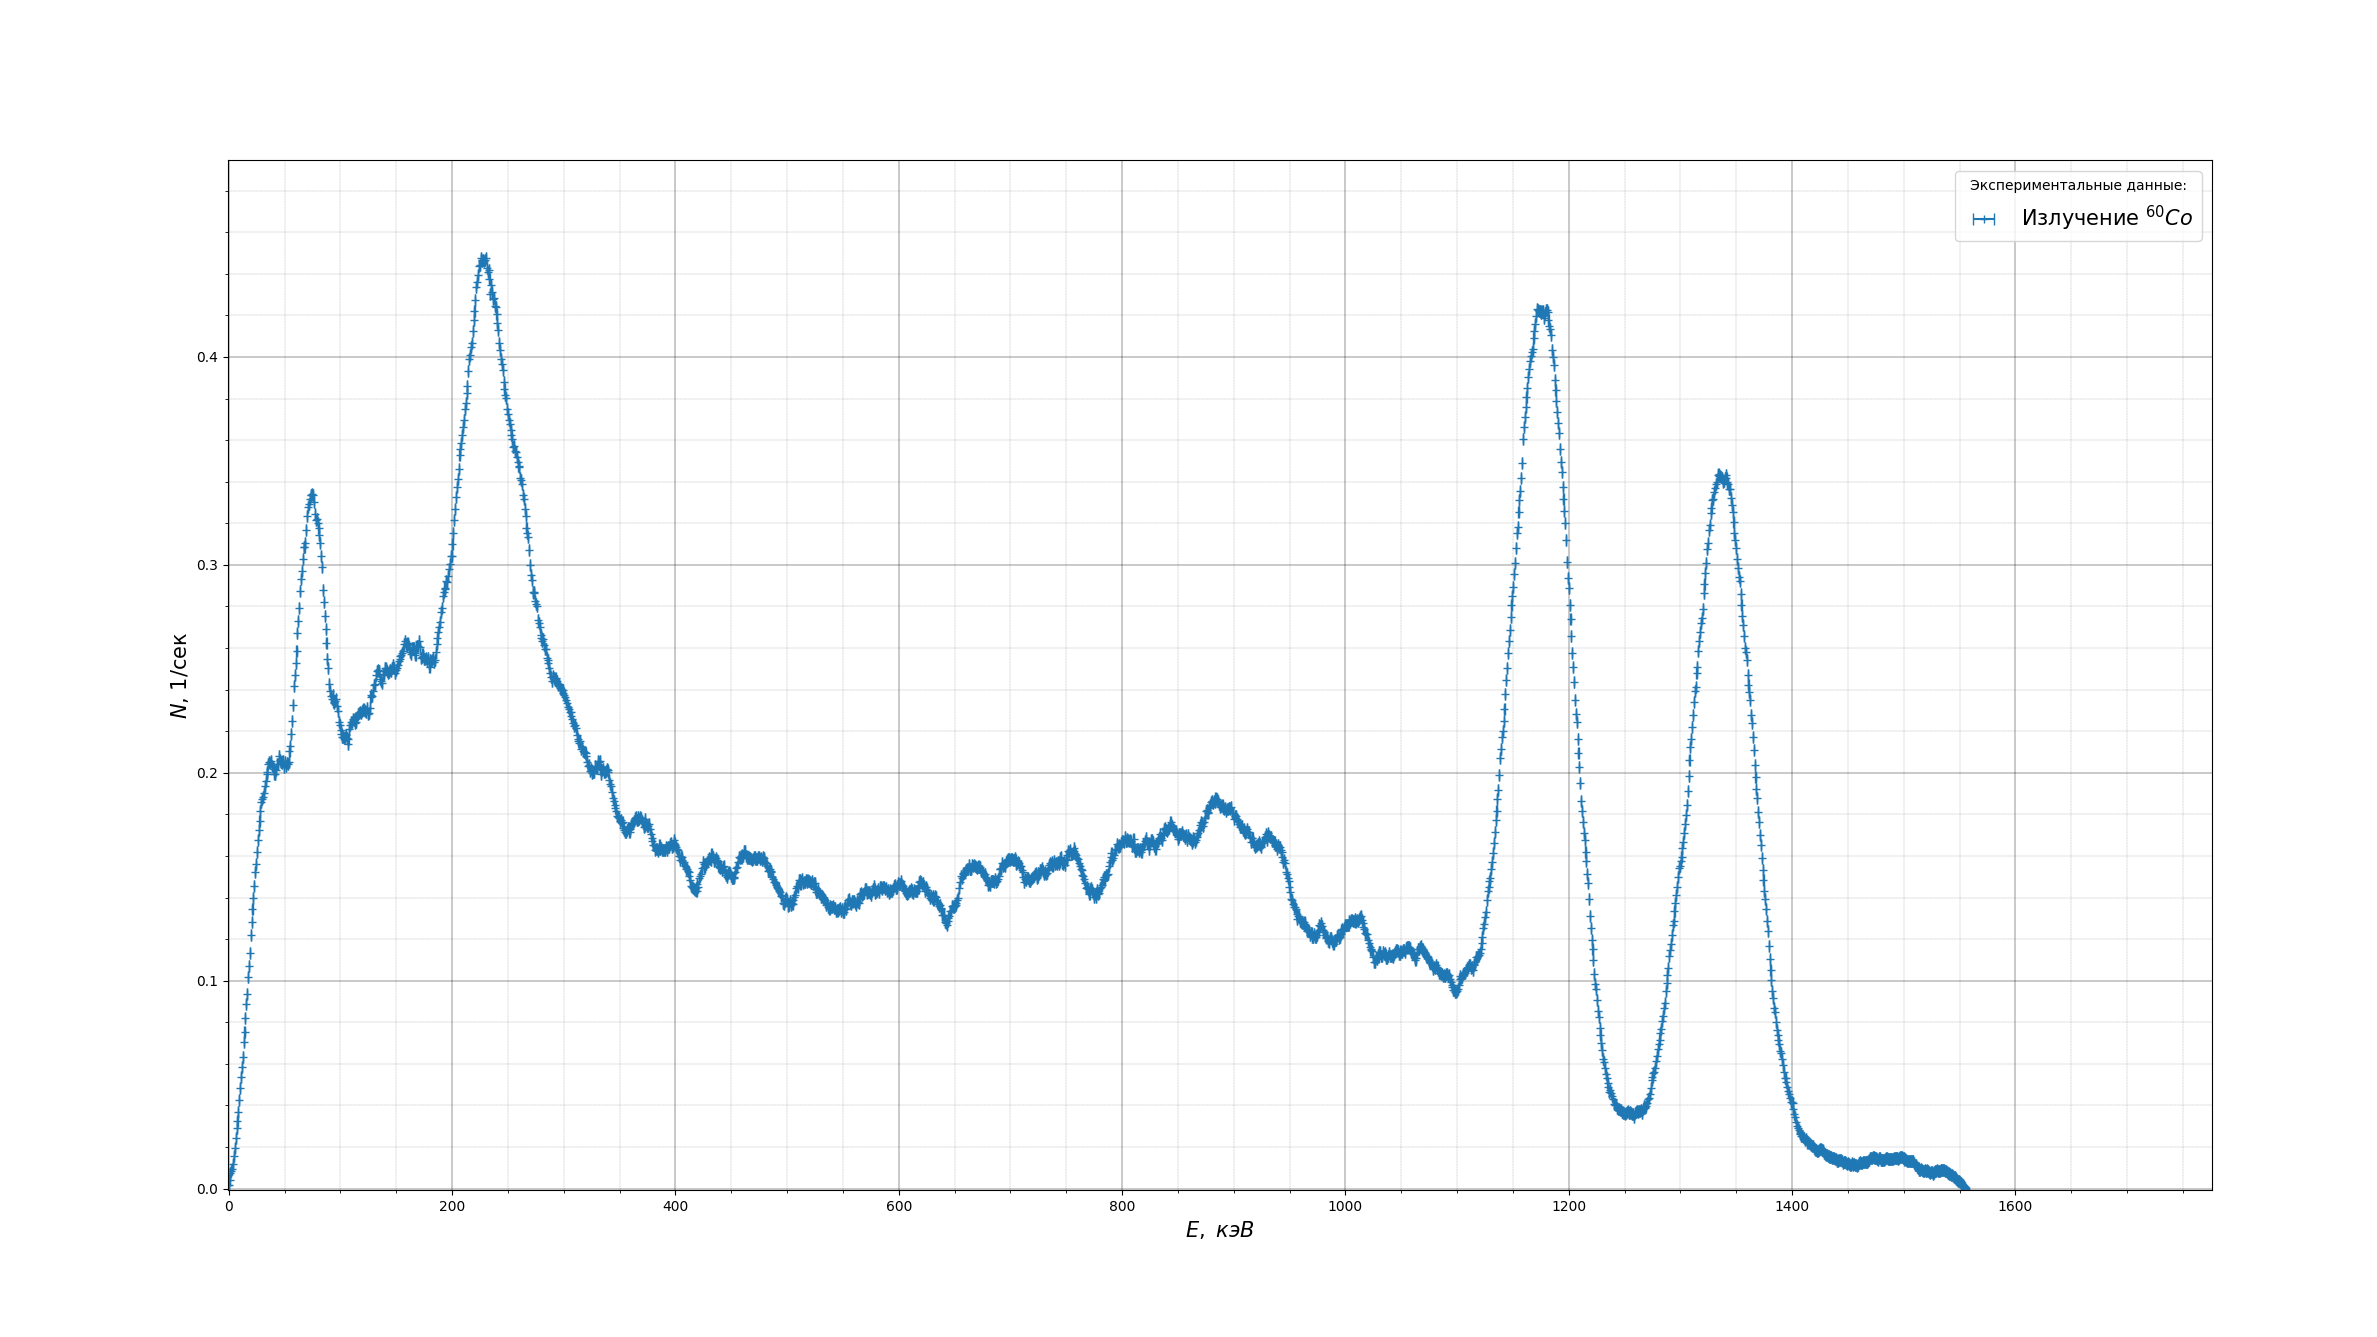
\includegraphics[width=0.95\linewidth]{Co_60}
		\caption{Спектр $^{60}Co$}
		\label{fig:co60}
	\end{figure}
	\begin{figure}[H]
		\centering
		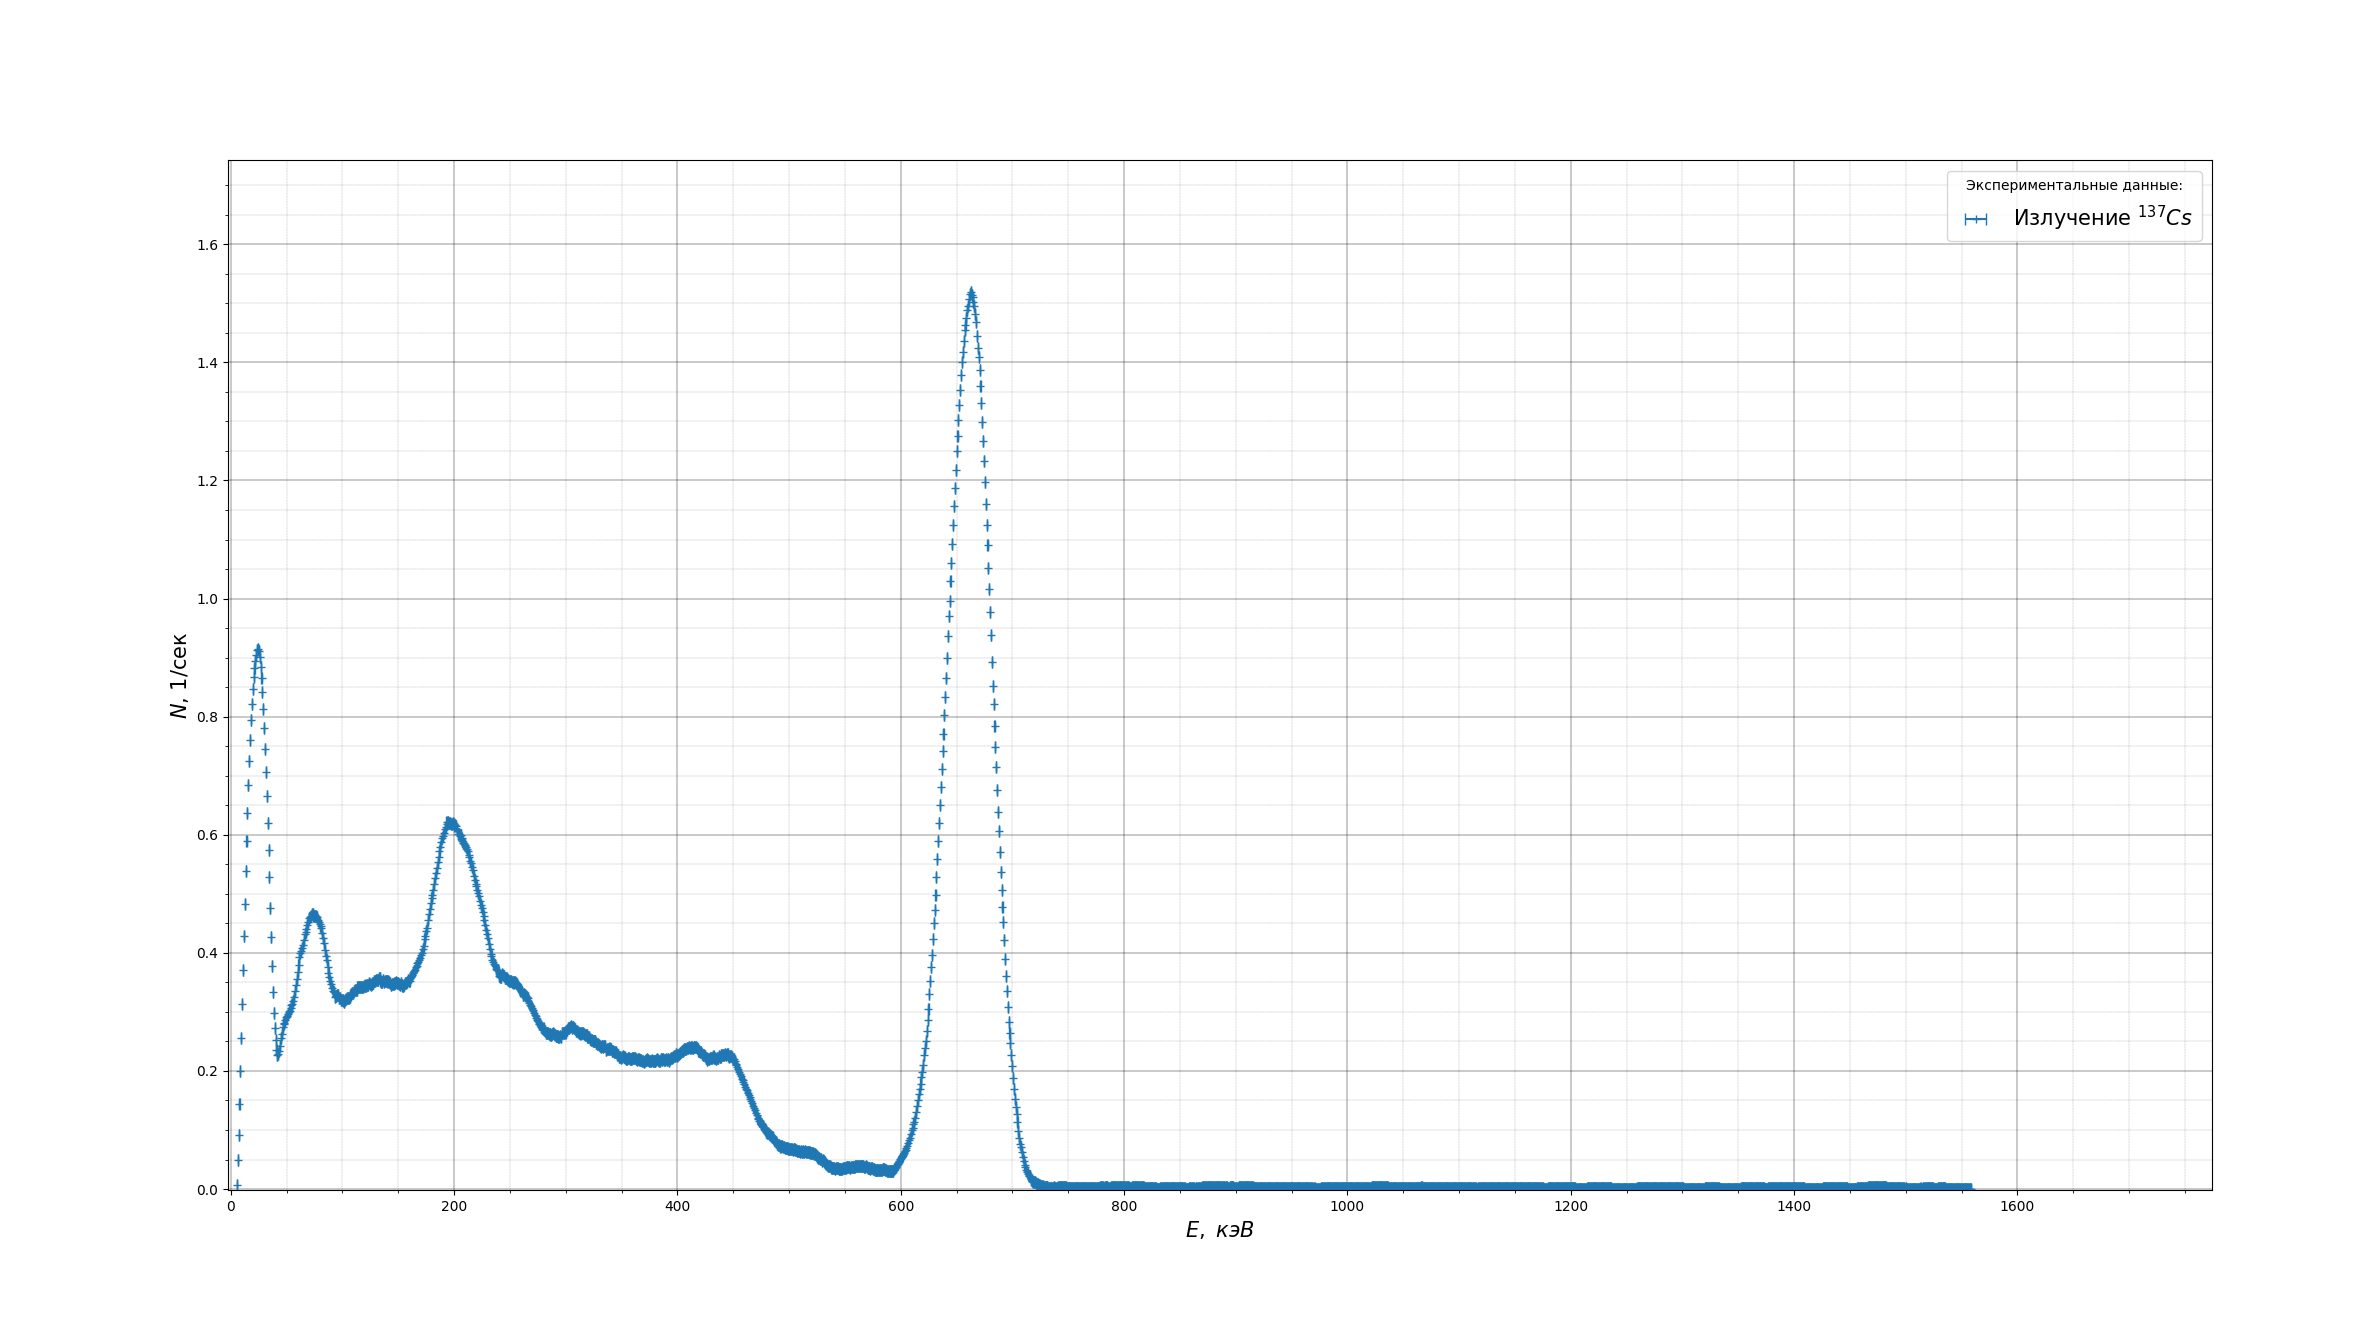
\includegraphics[width=0.95\linewidth]{Cs_137}
		\caption{Спектр $^{137}Cs$}
		\label{fig:cs137}
	\end{figure}
	Найдем пики прямого поглощения для изучаемых образцов. При помощи наложения нормального распределения с помощью цифровых средств найдем максимум в номере отсчета и переведем его в энергию по полученной ранее формуле.
	\begin{table}[H]
		\caption{Пики прямого поглощения}
		\begin{center}
			\begin{tabular}{|c|c|c|c|c|c|c|}
				\hline 
				Образец & $N_i $ & $ \Delta N_i $ & $ E_i, $ кэВ & $ \Delta E,_i $ кэВ  & $ R_i $ & $E_{\text{теор}}$, кэВ\\ 
				\hline 
				Натрий $ \mathrm{^{22}Na} $ & 718.1 & 42 & 508.8 & 40.2 & 0.079 & 511\\
				Натрий $ \mathrm{^{22}Na} $& 1695.2 & 76.6 & 1279.6 & 73.4 & 0.058 & 1275 \\
				Цезий $ \mathrm{^{137}Cs} $ & 915.3 & 47.4 & 664.2 & 45.3 & 0.069 & 661.6 \\
				Кобальт $ \mathrm{^{60}Co} $ & 1565.7 & 65.1 & 1177.0 & 62.3 & 0.053 & 1173\\
				Кобальт $ \mathrm{^{60}Co} $ & 1767.3 & 73.3 & 1336.5 & 70.2 & 0.053 & 1333 \\
				
				
				\hline 
			\end{tabular} 
		\end{center}
		\label{res}
	\end{table}

	\begin{table}[H]
		\caption{Комптновские спектры}
		\begin{center}
			\begin{tabular}{|c|c|c|c|}
				\hline 
				Образец & $ E_i, $ кэВ  & $ E_{c\; экс}, $ кэВ  & $ E_{c \; теор}, $ кэВ \\
				\hline 
				Натрий $ \mathrm{^{22}Na} $ & 508.8 & 320.2 & 341. \\
				Цезий $ \mathrm{^{137}Cs} $ & 664.2 & 483.2 & 477.2 \\
				Кобальт $ \mathrm{^{60}Co} $ & 1177.0 & 973.3 & 960.9 \\
				Натрий $ \mathrm{^{22}Na} $& 1279.6 & 1075.0 & 1062.3 \\
				\hline 
			\end{tabular} 
		\end{center}
		\label{compt}
	\end{table}
	
	\begin{table}[H]
		\caption{Пики обратного рассеяния}
		\begin{center}
			\begin{tabular}{|c|c|c|}
				\hline 
				Образец & $ E_i, $ кэВ  & $ E_{обр}, $ кэВ  \\
				\hline 
				Натрий $ \mathrm{^{22}Na} $  & 508.8 & 190 \\
				Цезий $ \mathrm{^{137}Cs} $ & 664.2 & 205 \\
				Кобальт $ \mathrm{^{60}Co} $ & 1336.5 & 230 \\
				\hline 
			\end{tabular} 
		\end{center}
		\label{obr}
	\end{table}
	\begin{figure}[H]
		\centering
		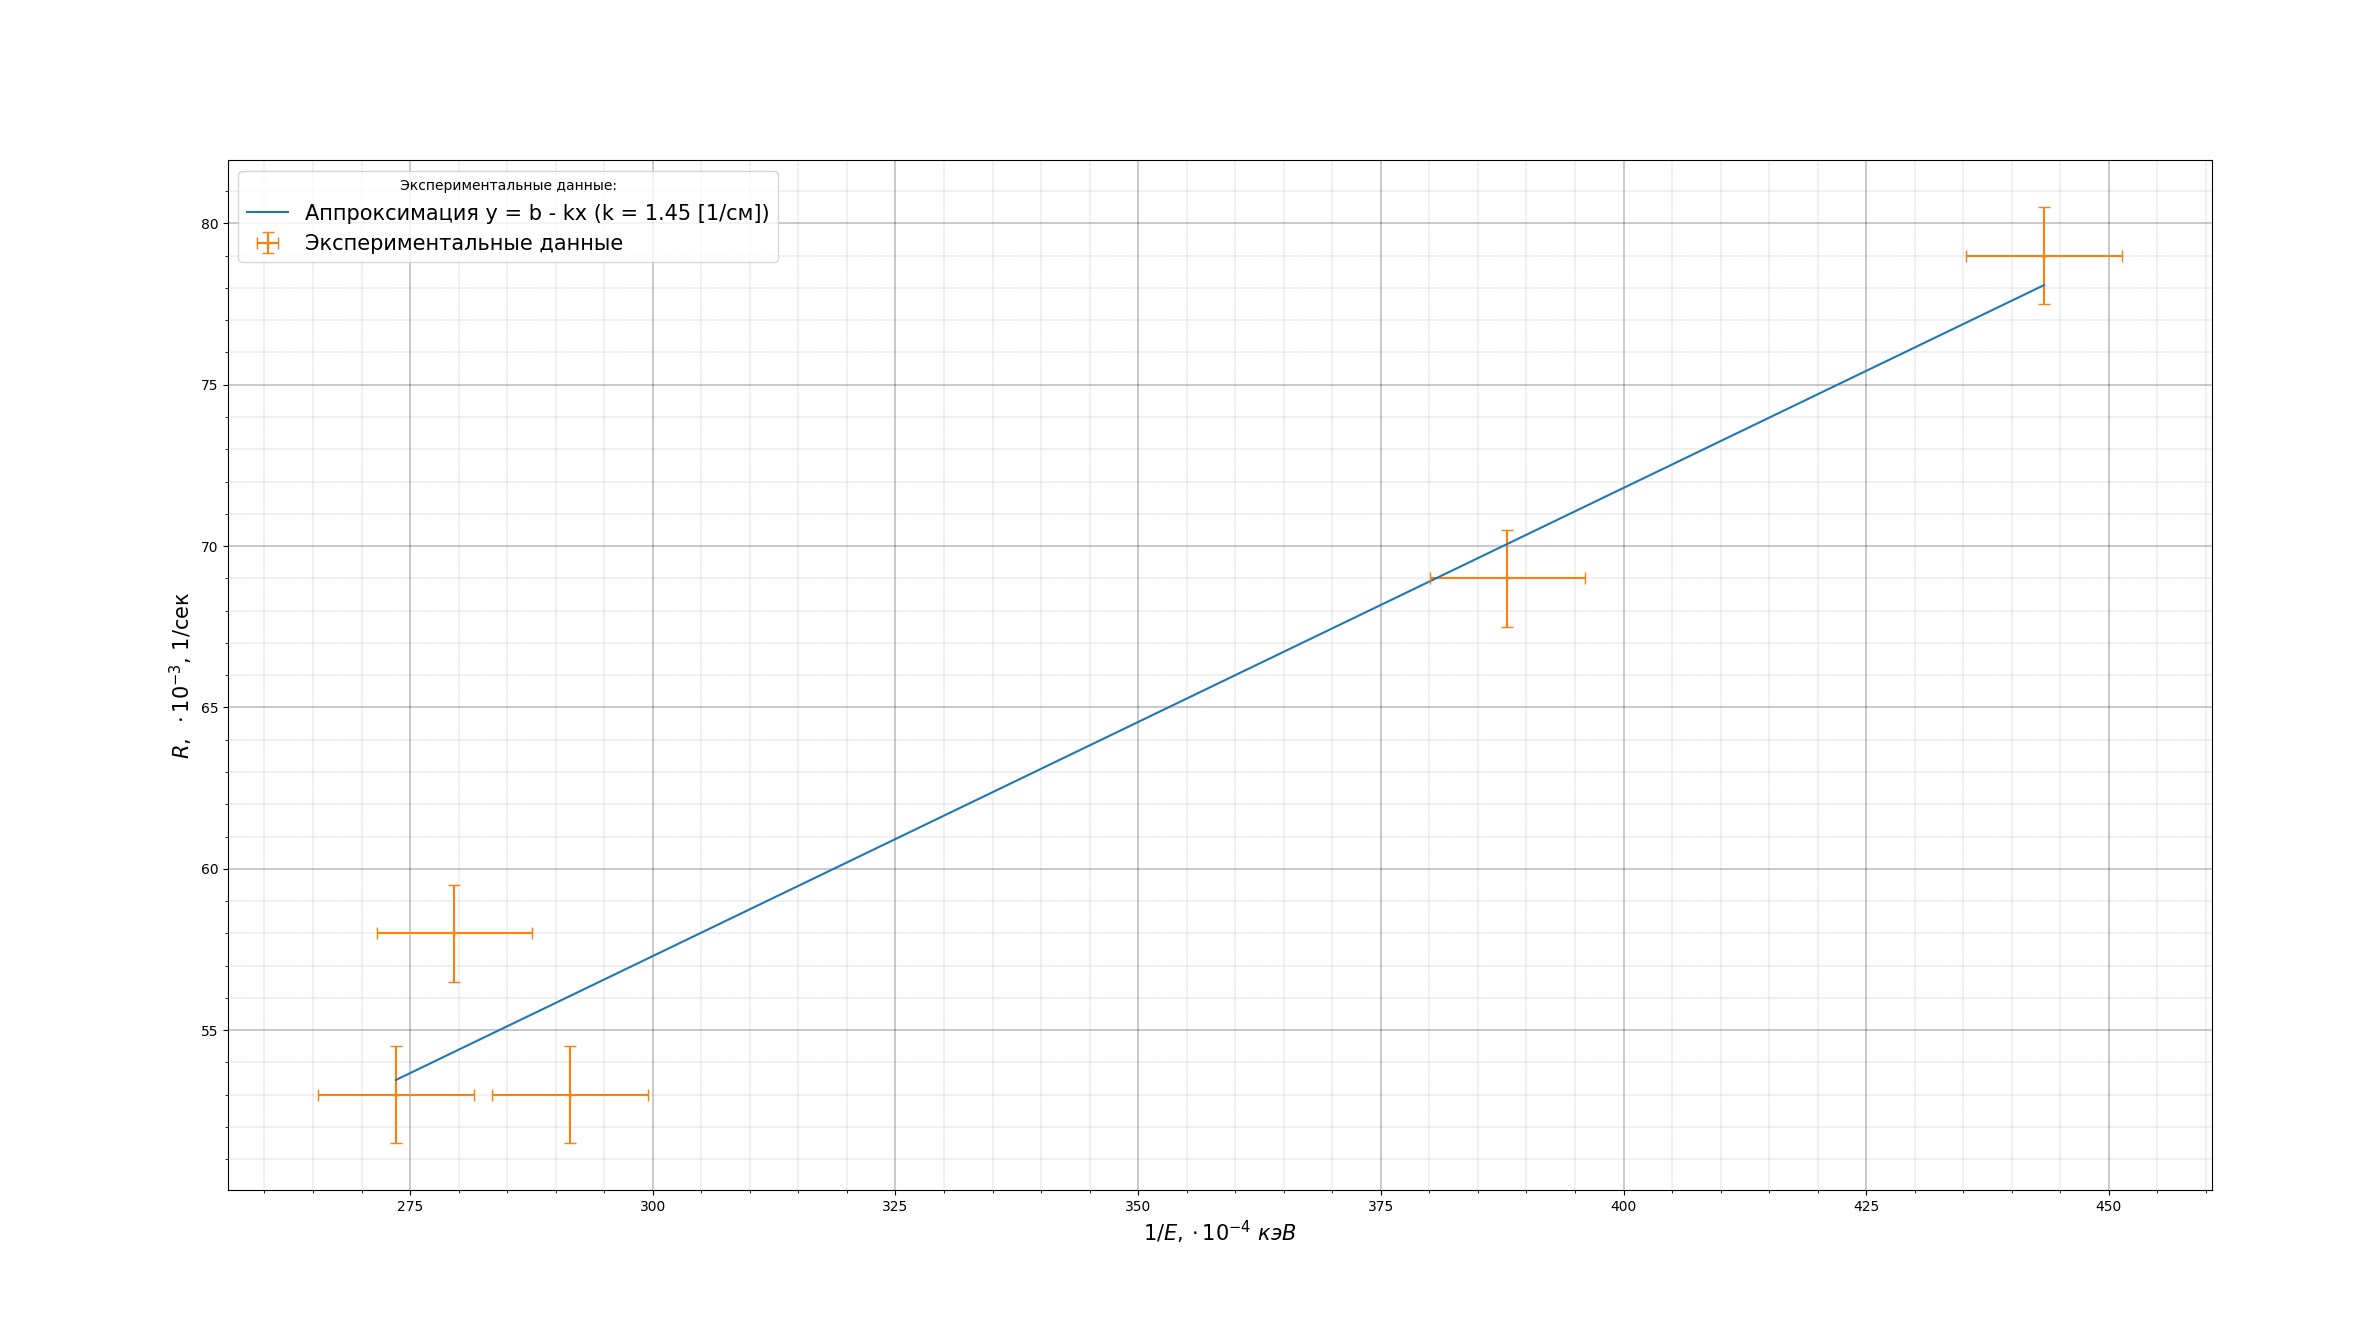
\includegraphics[width=0.95\linewidth]{R}
		\caption{Проверка формулы $ R = \dfrac{\mathrm{const}}{\sqrt{E}} $}
		\label{fig:r}
	\end{figure}
	\section{Вывод}
	В ходе работы после калибровки прибора были сняты спектры образцов $^{22}$Na,  $^{60}$Cо,  $^{137}Cs$ . В спектрах были исследованы пики, соответствующие следующим взаимодействиям гамма-квантов с веществом:
	\begin{itemize}
		\item фотоэффект (пики полного поглощения)
		\item эффект Комптона (характерное распределение энергий в спектре, оканчивающееся комптоновским краем)
		\item обратное рассеяние (пики обратного рассеяния)
		\item аннигиляция позитронов (пик 511 kэВ в спектре натрия, по которому проводилась калибровка)
	\end{itemize}
	
	Все значения энергии, опеределённые по спектрам, практически совпадали с табличными и расчётными. \par
	

\end{document}